\section{Characterizing Transnational Detours}
\label{datasets}
Here we discuss how we chose our vantage points within a country, and which servers to use as relays.  We also introduce our measurement methods for measuring which countries current Internet traffic is traversing to characterize transnational detours.

\subsection{Vantage Points}
To our knowledge, the publicly available traceroute datasets suitable for our goal are from iPlane~\cite{madhyastha2006iplane} and CAIDA (Center for Applied Internet Data Analysis)~\cite{caida}.  The iPlane project uses PlanetLab ~\cite{planetlab} nodes to run traceroutes to a random set of IP addresses that cover all BGP atoms.  This project also has historical data as far back as 2006.  Unfortunately, because iPlane uses PlanetLab nodes, which have been shown to mostly use the Global Research and Education Network (GREN), the traceroutes run from PlanetLab nodes will not be representative of typical Internet users' traffic paths~\cite{banerjee2004interdomain}.  The other publicly available dataset, from CAIDA, ran traceroutes from different vantage points around the world, but to randomized destination IP addresses that cover all /24s.  This is also not sufficient for what we wanted to measure because a typical Internet user is going to access a domain that will be locally resolved; the user will not input a specific IP address in their browser.  Therefore, we chose to run active measurements that would be most representative of an Internet user.  We chose to run DNS and traceroute measurements from RIPE Atlas probes, which are hosted all around the world and in many different settings, include home networks~\cite{ripe_atlas}.  The first advantage of using RIPE Atlas is that the probes can use the local DNS resolver, which would give us the best estimate of the traceroute destination.  The next advantage is that we can control the parameters of traceroute; we specified to use paris traceroute as well as conducting both ICMP and TCP traceroutes.  We discuss more of our parameter selection and methodology in Section~\ref{measure}.

Our study looks at the Alexa Top 100 domains in different countries, as well as the 3rd party domains that are requested as part of an original web request.  To obtain these 3rd party domains we {\tt curl} each of the Top 100 domains, but we must do so from within the country we are studying.  There is no current functionality to {\tt curl} from RIPE Atlas probes, so we established a VPN connection within each of these countries to {\tt curl} each domain and extract the 3rd party domains.

As one of our research goals is to quantify how well the use of an overlay network will help clients avoid surveillance, we need access to a set of relays.  We used eight Amazon EC2 instances, one in each geographic region (United States, Ireland, Germany, Singapore, South Korea, Japan, Australia, Brazil), as well as 4 VPS machines (France, Spain, Brazil, Singapore).  The conjunction of these two sets of machines allow us to evaluate surveillance avoidance with a geographically diverse set of relays.

\begin{figure*}
\centering
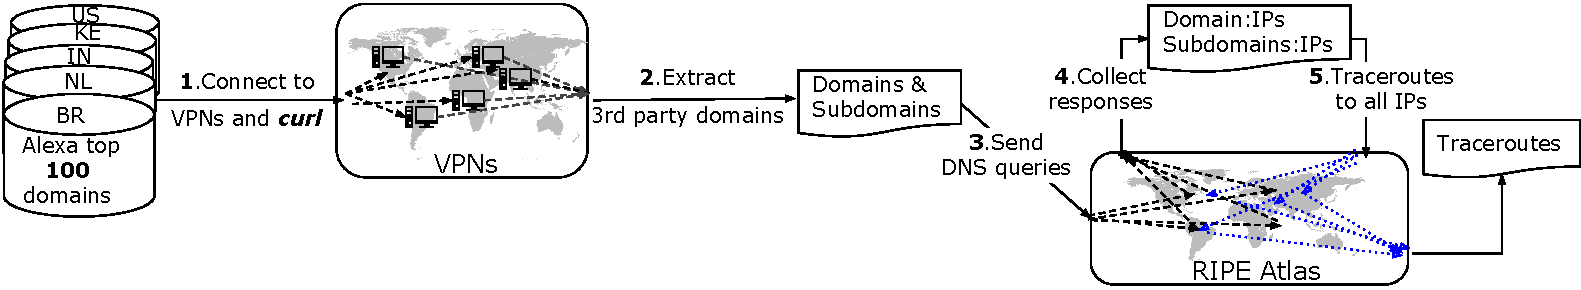
\includegraphics[width=.9\textwidth]{Current-Traffic_fig}
\caption{The measurement pipeline to study current traffic routes.}
\label{fig:pipeline1}
\end{figure*}

\begin{figure}
\centering
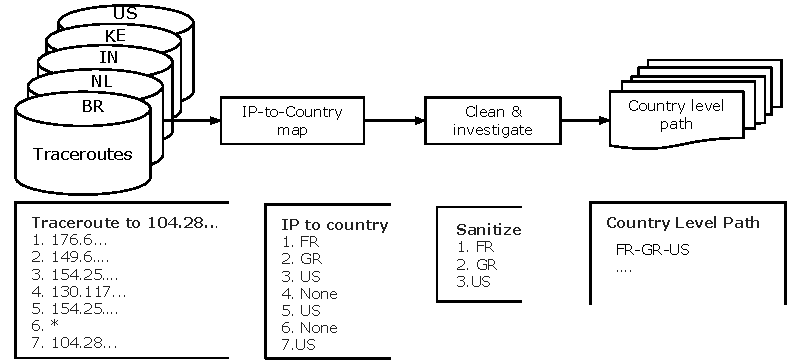
\includegraphics[width=.5\textwidth]{Analysis-Pipeline_fig}
\caption{The measurement pipeline to analyze traceroutes.}
\label{fig:analysis_pipeline}
\end{figure}

\subsection{Measurement Pipeline}
\label{pipeline}
{\bf Current Traffic.} Our methods for measuring where traffic paths go use the data-plane; we analyze the reported hops of traceroute measurements to find which countries are on the path from a client in Country X to a popular domain.  For this study, we used RIPE Atlas probes in Country X, specifically the set of probes that had unique ASes in the country.  The destinations for traceroutes are the Country X Alexa Top 100 domains, as well as the third party domains within the response bodies of the 100 domains.  There are three main steps to our measurement procedure: traceroute generation and collection, transformation of traceroutes to country-level paths, and path analysis.

\subsection{Results}

\newcommand{\headrow}[1]{\multicolumn{1}{c}{\adjustbox{angle=45,lap=\width-0.5em}{#1}}}
\newcolumntype{P}[1]{>{\raggedright\arraybackslash}p{#1}}
\begin{table*}[t]
\centering
\begin{tabular}{|P{37mm}|c|c|c|c|c|}
%\multicolumn{1}{l}{}    & \headrow{Host} & \headrow{Transit} & \headrow{Host} & \headrow{Transit} &\headrow{Host} &\headrow{Transit} &\headrow{Host}   &\headrow{Transit} &\headrow{Host}  &\headrow{Transit} \\
\hline
\textit{Country}    & \textit{Brazil}  & \textit{Netherlands}   & \textit{India} & \textit{Kenya} & \textit{United States}\\
\hline\hline
Brazil             &.169    &-     &-    & -  & - \\\hline\hline
Canada             &.001    &.007     &.015      &.006       & -  \\\hline
United States      &.774    &.454      &.629      &.443        &.969   \\\hline\hline
France             &.001    &.022      &.009      &.023       &.0013 \\\hline
Germany            &.002    &.013      &.014      &.028       &.0013  \\\hline
Great Britain      &.00006  &.019     &.021     &.032       &.0024 \\\hline
Ireland            &.016    &.064      &.027       &.108       &.0012   \\\hline
Netherlands        &.013    &.392      &.101      &.200      &.024  \\\hline
Spain              &.001    &-     & -    &  -     &-   \\\hline\hline
Kenya              &-        &  -    & -    &.022        &-  \\\hline
Mauritius          &  -      & -    & -   &.004       & -  \\\hline
South Africa       & -       & -     & -  &.021       &- \\\hline\hline
United Arab Emirates & -     & -     & -   &.011        &-  \\\hline
India              &  -      & -     &.053    &.002        &-  \\\hline
Singapore          & -       &.002     &.103      &.027       & - \\\hline
\end{tabular}
\caption{Fraction of paths that end in each country in default routes.}
\label{tab:host}
\end{table*}

\begin{table*}[t]
\centering
\begin{tabular}{|P{37mm}|c|c|c|c|c|}
%\multicolumn{1}{l}{}    & \headrow{Host} & \headrow{Transit} & \headrow{Host} & \headrow{Transit} &\headrow{Host} &\headrow{Transit} &\headrow{Host}   &\headrow{Transit} &\headrow{Host}  &\headrow{Transit} \\
\hline
\textit{Country}    & \textit{Brazil}  & \textit{Netherlands}   & \textit{India} & \textit{Kenya} & \textit{United States}\\
\hline\hline
Brazil              &1.00       & -   & -     & -     & -\\\hline\hline
Canada                &.013       &.007     &.016       &.008      &.081 \\\hline
United States                 &.844        &.583     &.715      &.616       &1.0 \\\hline\hline
France                 &.059     &.102      &.104       &.221      &.104 \\\hline
Germany                 &.005       &.050    &.032      &.048      &.008 \\\hline
Great Britain                &.024       &.140     &.204      &.500      &.006 \\\hline
Ireland                &.028       &.106      &.031     &.133      &.006 \\\hline
Netherlands                 &.019        &1.0      &.121      &.253      &.031 \\\hline
Spain                  &.176       &.004     & -     & -      &- \\\hline\hline
Kenya                 & -       &-    & -      &1.0      &- \\\hline
Mauritius                  & -       & -     & -      &.322       &- \\\hline
South Africa                 &-        & -    & -     &.334       &- \\\hline\hline
United Arab Emirates                  &.00003        & -    & -     &.152       &- \\\hline
India               &  -    &.0007    &1.0     &.058     &.0005 \\\hline
Singapore                 &.0009        &.002     &.270       &.040       &.003 \\\hline
\end{tabular}
\caption{Fraction of paths that each country transits in default routes.}
\label{tab:transit}
\end{table*}

Table \ref{tab:host} shows the five studied countries along the top of the table, and the countries that host their traffic along the Y axis.  For example, the United States is the endpoint of 84\% of the paths that originate in Brazil.  Table \ref{tab:transit} shows the fraction of paths that transit certain countries (along the Y axis).  The methods we use are described in Section \ref{pipeline1}, and in this section we discuss our findings.

{\bf Hosting Diversity}
First we look at hosting diversity.  This shows us how many unique countries in which a domain is hosted -- the more countries that a domain is hosted in creates a greater chance that the content is replicated in a favorable country, and could potentially allow a client to circumvent an unfavorable country.  By querying DNS from 26 vantage points around the world, we found that there is hosting diversity among the Alexa Top 100 Domains.  About half of the Alexa Top 100 Domains in each of the five countries studied are hosted in more than one country.  This can be seen in Figure~\ref{fig:host_diversity}.  We see there are two distinct modes in the graph, one representing the domains that are hosted in a single country, and the other mode representing CDNs.  This shows that many domains are hosted in a single unique country, which leads us to our next analysis - where are these domains hosted, and which countries are traversed on the way to reach these locations.

\begin{figure}
\centering
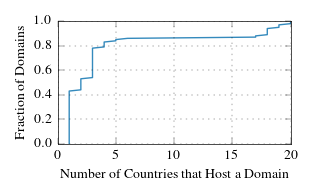
\includegraphics[width=.5\textwidth]{domain_hist_US}
\caption{The number of Alexa Top 100 US Domains hosted in different countries.}
\label{fig:host_diversity}
\end{figure}

{\bf Surveillance States Host Domains}
The most common destination among all five countries studied is the United States: 77\%, 45\%, 63\%, 44\%, and 97\% of paths originating in Brazil, Netherlands, India, Kenya and the United States, respectively, are currently reaching content located in the United States. Despite the amount of country-level hosting diversity, we see the majority of paths from all five countries ending in a single country.  The fraction of paths that are hosted in various countries can be seen in Table~\ref{tab:host} (the complete table can be seen in the Appendix).  This is significant because the United States is a known surveillance state, and therefore these percentages represent just a portion of foreign traffic that the United States can conduct surveillance on.  Our results also show the Netherlands as a common hosting location for traffic originating in the Netherlands, India, and Kenya.

For Indian traffic, in addition to the 63\% hosted in the United States and the 10\% hosted in the Netherlands, another 10\% is hosted in Singapore.  This can best be explained by the number of underwater cables with landing points in both India and Singapore~\cite{cablemap}.  More specifically, there is a cable that directly connects Chennai, India and Changi North, Singapore, and is owned by Tata Communications, which is one of the top global Internet providers (in terms of transitted IP space)~\cite{bakers}.  

For Kenyan traffic, the United States hosts 44\% of the content, but Ireland hosts 10\%; Ireland is a popular hosting location for U.S. companies due to it's relaxed enforcement of privacy in the private sector.  

All of the countries studied (except for the United States) host a small percentage of their own traffic.  For traffic that originates in Brazil, only 17\% of it also ends in Brazil.  Only 5\% and 2\% of Indian and Kenyan traffic, respectively, end in the originating country.  

Only a fraction of country code top-level domains are hosted with in the respective country.  For Kenya, 24 of the Top 100 Domains are .ke domains, and of these 24 domains only 5 are hosted within Kenya.  29 out of 40 .nl domains are hosted in the Netherlands; 4 of 13 .in domains are hosted in India; 18 of 39 .br domains are hosted in Brazil.  Interestingly, all .gov domains were hosted in their respective country.

{\bf Traffic Transits Surveillance States}
Similar to the trend of hosting domains, the United States also transits a large portion of foreign traffic -- it transits a larger portion of traffic than it hosts.  Brazilian traffic traverse the United States on 84\% of the paths; therefore, the United States can conduct surveillance on 84\% of the traffic originating in Brazil, despite Brazil's strong efforts in avoiding United States surveillance.  Even though India and Kenya are geographically distant, 72\% and 62\% of their traffic transits the United States.  Of the five countries studied, the Netherlands has the lowest percentage of traffic that transits the United States at 58\%.  

Great Britain and the Netherlands are on the path for a significant percentage of traffic originating in India and Kenya.  50\% and 20\% of paths that originate in Kenya and India transit Great Britain.  Traffic that traverses the Netherlands can be explained by the large IXP located there; traffic that traverses Great Britain is likely due to being on the path between the originating country and the final destination in a European country.

Mauritius, South Africa, and the United Arab Emirates transit 32\%, 33\%, and 15\% of traffic from Kenya.  There are direct underwater cables from Kenya to Mauritius, and from Mauritius to South Africa.  Additionally, there is a cable from Mombasa, Kenya to Fujairah, United Arab Emirates.  This accounts for the large percentages of traffic that pass through these countries.

{\bf Tromboning Traffic Transits Surveillance States}
As mentioned in Section \ref{trend1}, the percentage of domestic traffic in some of the countries studied is extremely small.  For India, only 5\% of traffic is domestic and for Kenya, 2\% is domestic; despite the small amount of domestic traffic, some of this traffic trombones.  This can be seen better in the cases of Brazil and the Netherlands; figure \ref{fig:trombone_netherlands} shows the amount of paths that trombone to differing countries for the Netherlands.

\begin{figure*}[!htb]
\minipage{0.32\textwidth}
  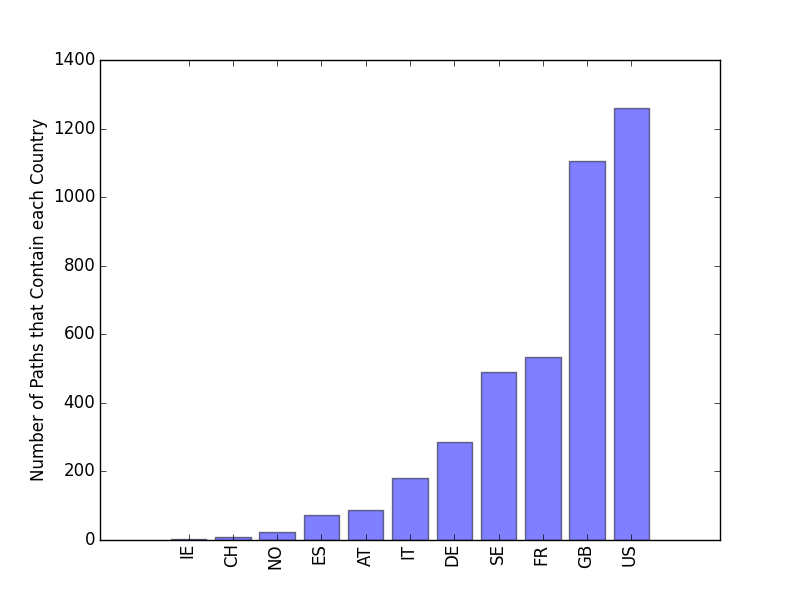
\includegraphics[width=\linewidth]{nl_trombone_new}
  \caption{The countries that tromboning Netherlands traffic transits.}\label{fig:trombone_netherlands}
\endminipage\hfill
\minipage{0.32\textwidth}
  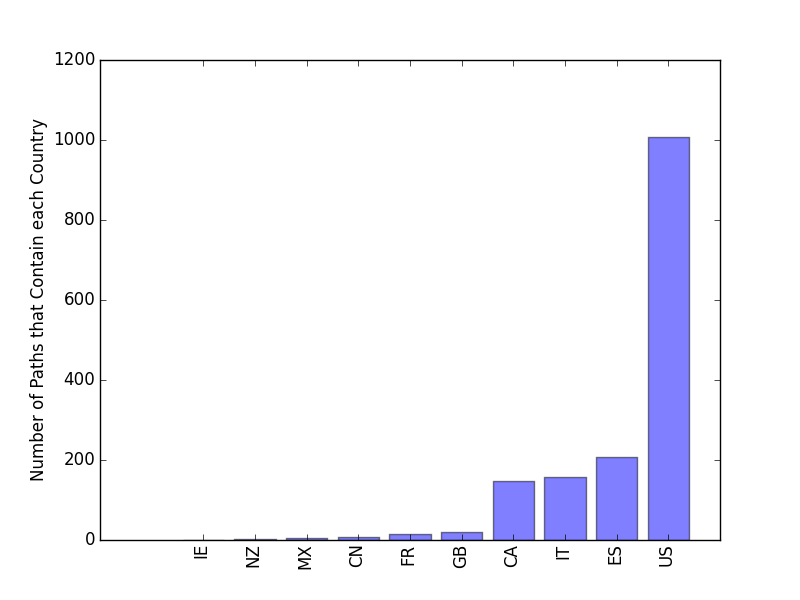
\includegraphics[width=\linewidth]{br_trombone_new}
  \caption{The countries that tromboning Brazilian traffic transits.}\label{fig:trombone_brazil}
\endminipage\hfill
\minipage{0.32\textwidth}%
  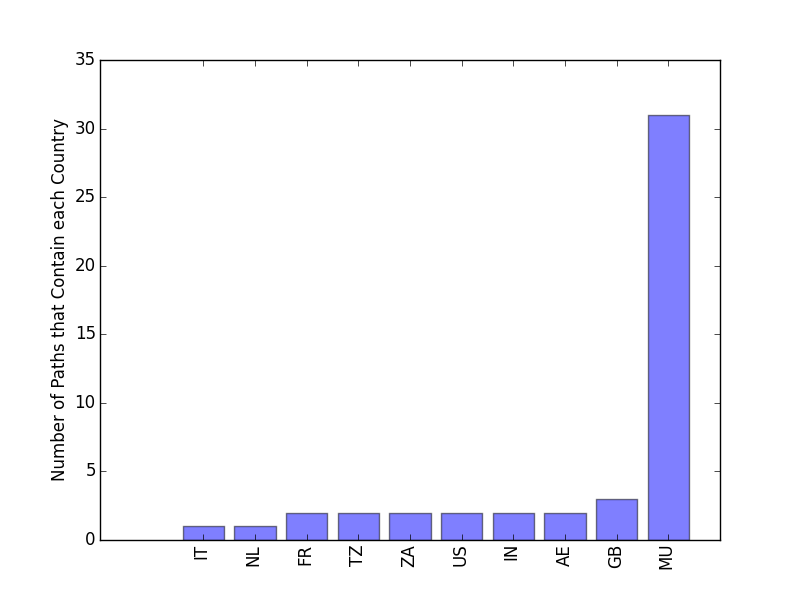
\includegraphics[width=\linewidth]{ke_trombone_new}
  \caption{The countries that tromboning Kenyan traffic transits.}\label{fig:trombone_kenya}
\endminipage
\end{figure*}

%\begin{figure}
%\centering
%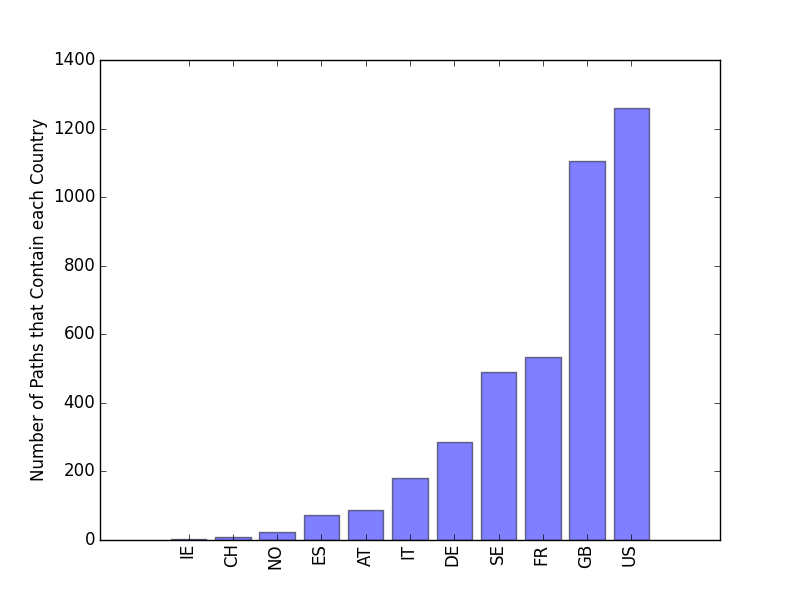
\includegraphics[width=.5\textwidth]{nl_trombone_new}
%\caption{The countries that tromboning Netherlands traffic transits.}
%\label{fig:trombone_netherlands}
%\end{figure}

24\% of all paths originating in the Netherlands (62\% of domestic traffic) trombone to a foreign country before returning to the Netherlands. The most common countries traffic trombones to are the United States and Great Britain.  Traffic that should be kept local is susceptible to surveillance because it transits two well-known surveillance states.  For Brazil, 5\% of all traffic starts in the Netherlands, transits a foreign country, and returns to the Netherlands (30\% of domestic traffic trombones).  The most common country traffic trombones to is the United States. 

{\bf United States as an Outlier}
Most of the results discussed thus far have shown that Brazilian, Netherlands, Indian, and Kenyan traffic often transit surveillance states, most notable the United States.  The results from studying traffic that originates in the United States are drastically different from those of the other four countries.  The other four countries hosted very small amounts of their own traffic, whereas the United States hosts 97\% of the content that is accessed from within the country.  Only 13 unique countries are ever on a path from the United States to a domain in the Top 100 (or third party domain), whereas 30, 30, 25, and 38 unique countries are seen on the paths originating in Brazil, Netherlands, India, and Kenya.  There are only 6 foreign countries that host content for traffic originating in the United States, and the fraction of content hosted in these countries is less than 4\% combined.

\subsection{Limitations}
The measurement methods described in Section~\ref{datasets} are not without limitations.  First, our study is solely based on IPv4 routes, which likely differ from IPv6 routes.  Here we also discuss limitations with geolocation accuracy, path asymmetry, and traceroute completeness.

\subsubsection{IPv4}
The measurements we conducted only collect and analyze IPv4 paths, and therefore all IPv6 paths are left out of our study.  IPv6 paths likely differ from IPv4 paths as not all routers that support IPv4 also support IPv6.  Future work includes studying IPv6 paths and which countries they transit, as well as a comparison of country avoidability between IPv4 and IPv6 paths. 

\subsubsection{Country Mapping}
Previous work has shown that there are fundamental challenges in deducing a geographic location from an IP address, despite using different methods such as DNS names of the target, network delay measurements, and host-to-location mapping in conjunction with BGP prefix information~\cite{padmanabhan2001investigation}.  Because the focus of this work is on measuring and avoiding surveillance, and not on geolocation algorithms, we used a pre-existing geolocation service: MaxMind~\cite{maxmind}.

Geolocation services and tools have been studied and proposed, and continue to be a growing research area.  We use MaxMind's geolocation service to map IP addresses to their respective countries.  While it has been shown that there are inaccuracies and incompleteness in MaxMind's data, research has also shown that other geolocation tools have similar or worse inaccuracy rates~\cite{huffaker2011geocompare}.  To address the incompleteness of the data, we cleaned up our IP to country mapping by removing all IP addresses that resulted in a `None' response when querying MaxMind.  This method provides a lowerbound on the number of countries that are included on the path, and therefore a lowerbound on the countries that can conduct surveillance.  

\subsubsection{Path Asymmetry}
Previous work has shown that paths are not symmetric most of the time -- the forward path from point A to point B does not match the reverse path from point B to point A~\cite{he2005routing}.  Most work on path asymmetry has been done at the AS level, but not at the country level.  Our measurement methods only take the forward path (from client to domain or relay) into account, and not the path from the domain or relay to the client.  

We conducted a study to measure path asymmetry at the country granularity; if country-level paths are symmetric, then the results of our measurements would be representative of the forward {\it and} reverse paths, but if the country-level paths are asymmetric, then our measurement results only provide a lowerbound on the number of countries that could potentially conduct surveillance.  Using 100 RIPE Atlas probes located around the world, and 8 Amazon EC2 instances, we ran traceroute measurements from every probe to every EC2 instance and from every EC2 instance to every probe.  After geolocating the IPs to countries, we analyzed the paths for symmetry.  First, we compared the set of countries on the forward path to the set of countries on the reverse path; this yielded about 30\% symmetry.  What we wanted to know is whether or not the reverse path has more countries on it than the forward path.  We measured how many reverse paths were a subset of the respective forward path; this was the case for 55\% of the paths.  

The results of this measurement are not convincing enough to state that country-level paths are symmetric, and therefore our measurements and results represent a lowerbound on the number of countries that transit traffic; our results are a lowerbound on how many unfavorable countries transit a client's traffic.

\subsubsection{Traceroute Accuracy and Completeness}
Our study is limited by the accuracy and completeness of traceroute.  Research has shown that there are a number of anomalies that can occur in traceroute-based measurements~\cite{augustin2006avoiding}, but most traceroute anomalies do not cause an overestimation in surveillance states.  The incompleteness of traceroutes, where a router does not respond, causes our results to be an underestimation of the number of surveillance states, and therefore also provides a lowerbound on surveillance.
